\subsection{Vue d'ensemble de \touist}\label{sec:sat_interface}

\touist est composé de trois modules, mais l'utilisateur standard ne verra que l'un d'entre eux : l'interface. Dans la suite nous insistons principalement sur cette dernière plutôt que sur le traducteur et le solveur. L'architecture globale est illustrée par la figure~\ref{fig:archi-simple-touist}.

\begin{figure}[!ht] \centering
  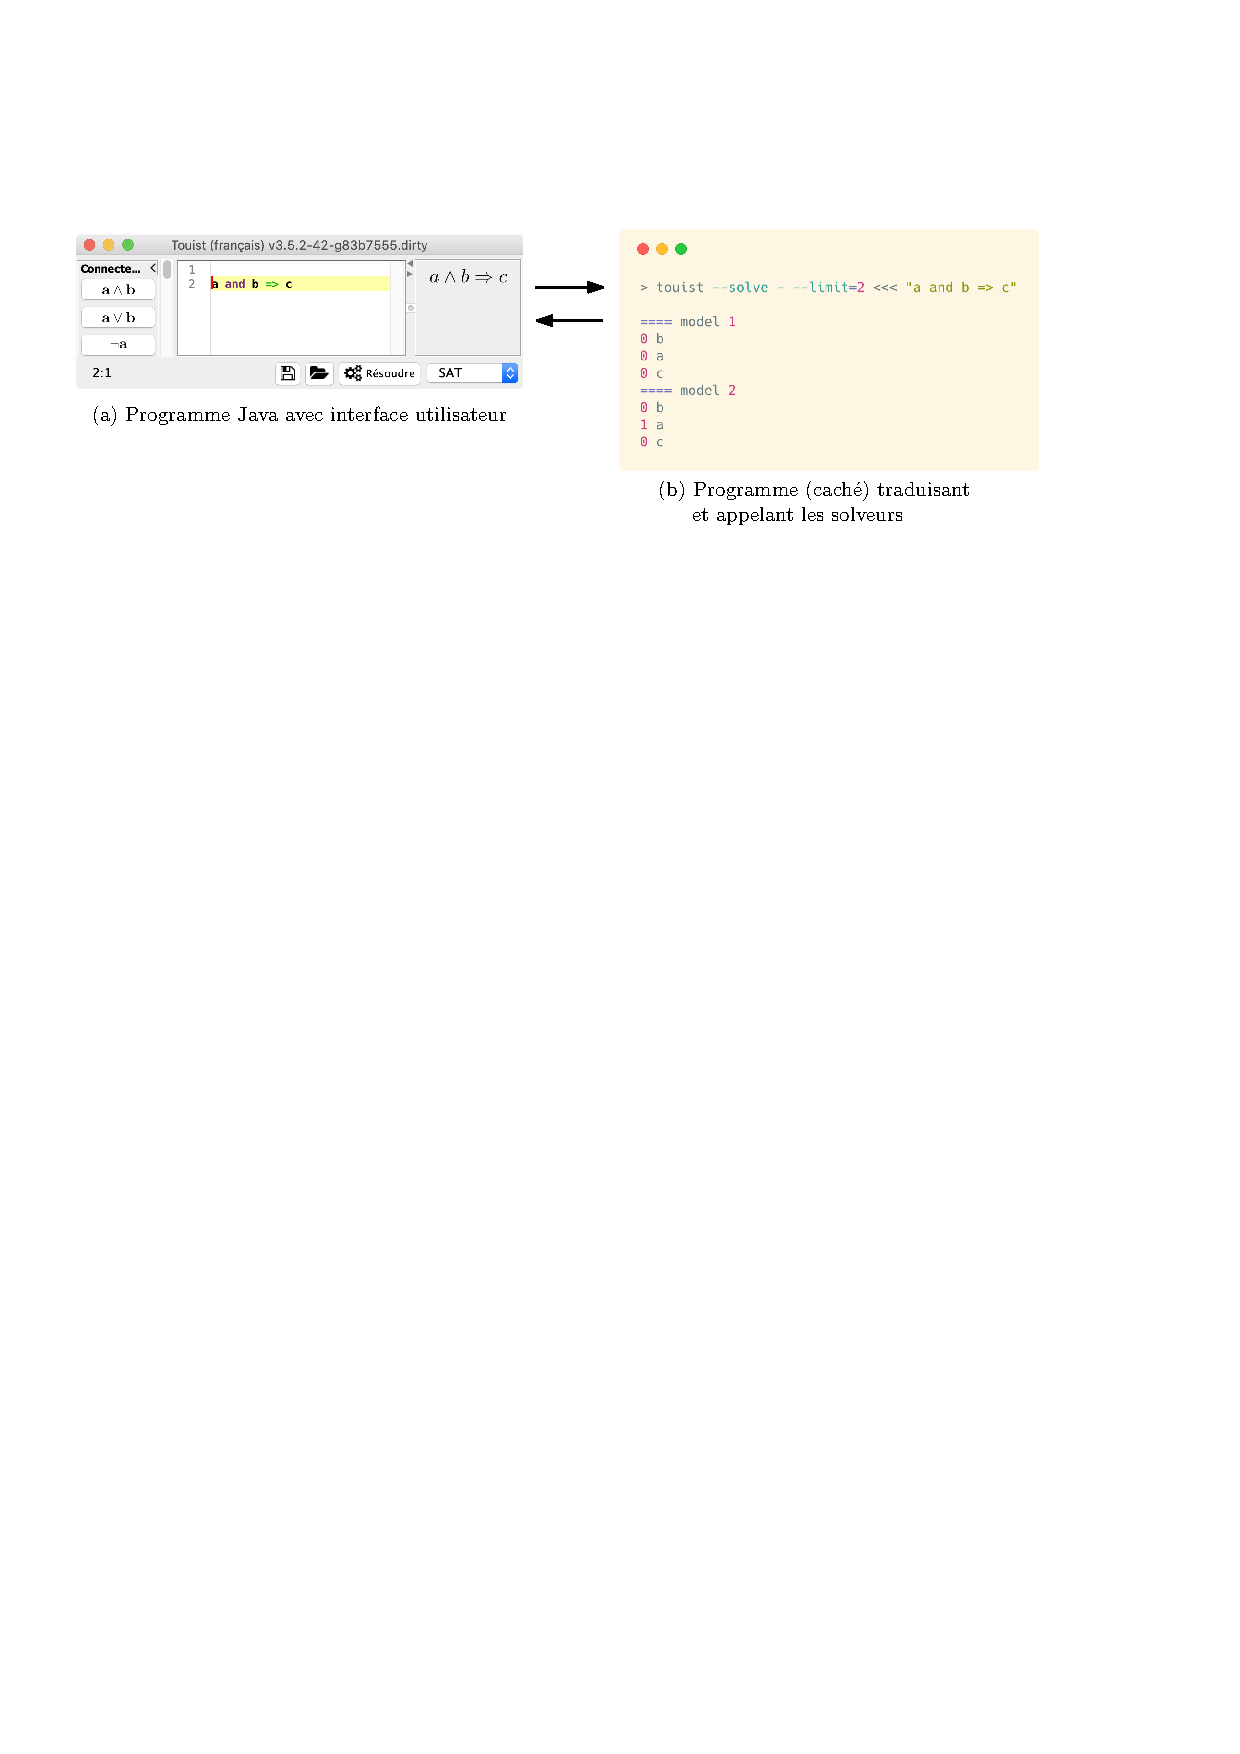
\includegraphics[width=1\textwidth]{figures/archi-simple}
  \caption{Architecture simplifiée de \touist. L'interface graphique écrite en Java fait appel à un programme en ligne de commande écrit en OCaml pour traduire et résoudre les problèmes.} \label{fig:archi-simple-touist} 
\end{figure}

Avec \touist , on accède à un éditeur puissant et convivial pour éditer des formules logiques complexes et des contraintes variées comme :

\[\bigwedge_{i \in \{1..9\}} (P_i \IMPL Q_{i+1})\]

\noindent
qui s'écrira simplement en \touist :
% bash ./scripts/touist-to-latex-et-verbatim.sh <<< 'bigand $i in [1..9]: P(i) => Q(i+1) end'
\begin{mdpre}%mdk
\noindent{\mdcolor{navy}bigand}~{\mdcolor{purple}\$i}~{\mdcolor{navy}in}~{}[{\mdcolor{purple}1}..{\mdcolor{purple}9}]:\\
~~~~P(i)~=\textgreater{}~Q(i+{\mdcolor{purple}1})\\
{\mdcolor{navy}end}%mdk
\end{mdpre}%mdk

\noindent
qui abrège confortablement :\\

\[(P_1 \Rightarrow Q_2) \AND (P_2 \IMPL Q_3) \AND \ldots (P_9\IMPL Q_{10}).\] 
\\

%%%%%%%%%%%%%%%%%%%%%%%%%%%%%%%

Une fois qu'une formule a été donnée à l'interface, sa satisfiabilité peut être vérifiée : l'interface peut l'envoyer au solveur qui retourne, s'il existe, un modèle. %, affiché comme le montre la figure \ref{fig:capture-modeles} si un tel modèle existe. 
Ensuite, par l'intermédiaire de l'interface, l'utilisateur peut, par exemple, demander d'autres modèles (bouton \enquote{Next} de l'interface). Contrairement à \satoulouse qui aurait nécessité de modifier les formules pour interdire le modèle et de relancer le solveur, \touist conserve une instance du solveur en attente, ce qui permet d'obtenir les modèles suivants bien plus rapidement.

Les modèles renvoyés par le solveur sont totaux : une valeur est affectée à chacune des variables apparaissant dans les formules envoyées au solveur. L'utilisateur peut sélectionner uniquement les propositions vraies ou les propositions fausses. Il peut également sélectionner des sous-ensembles de variables en tapant une expression régulière pour les filtrer.


\begin{figure}[!ht] \centering
  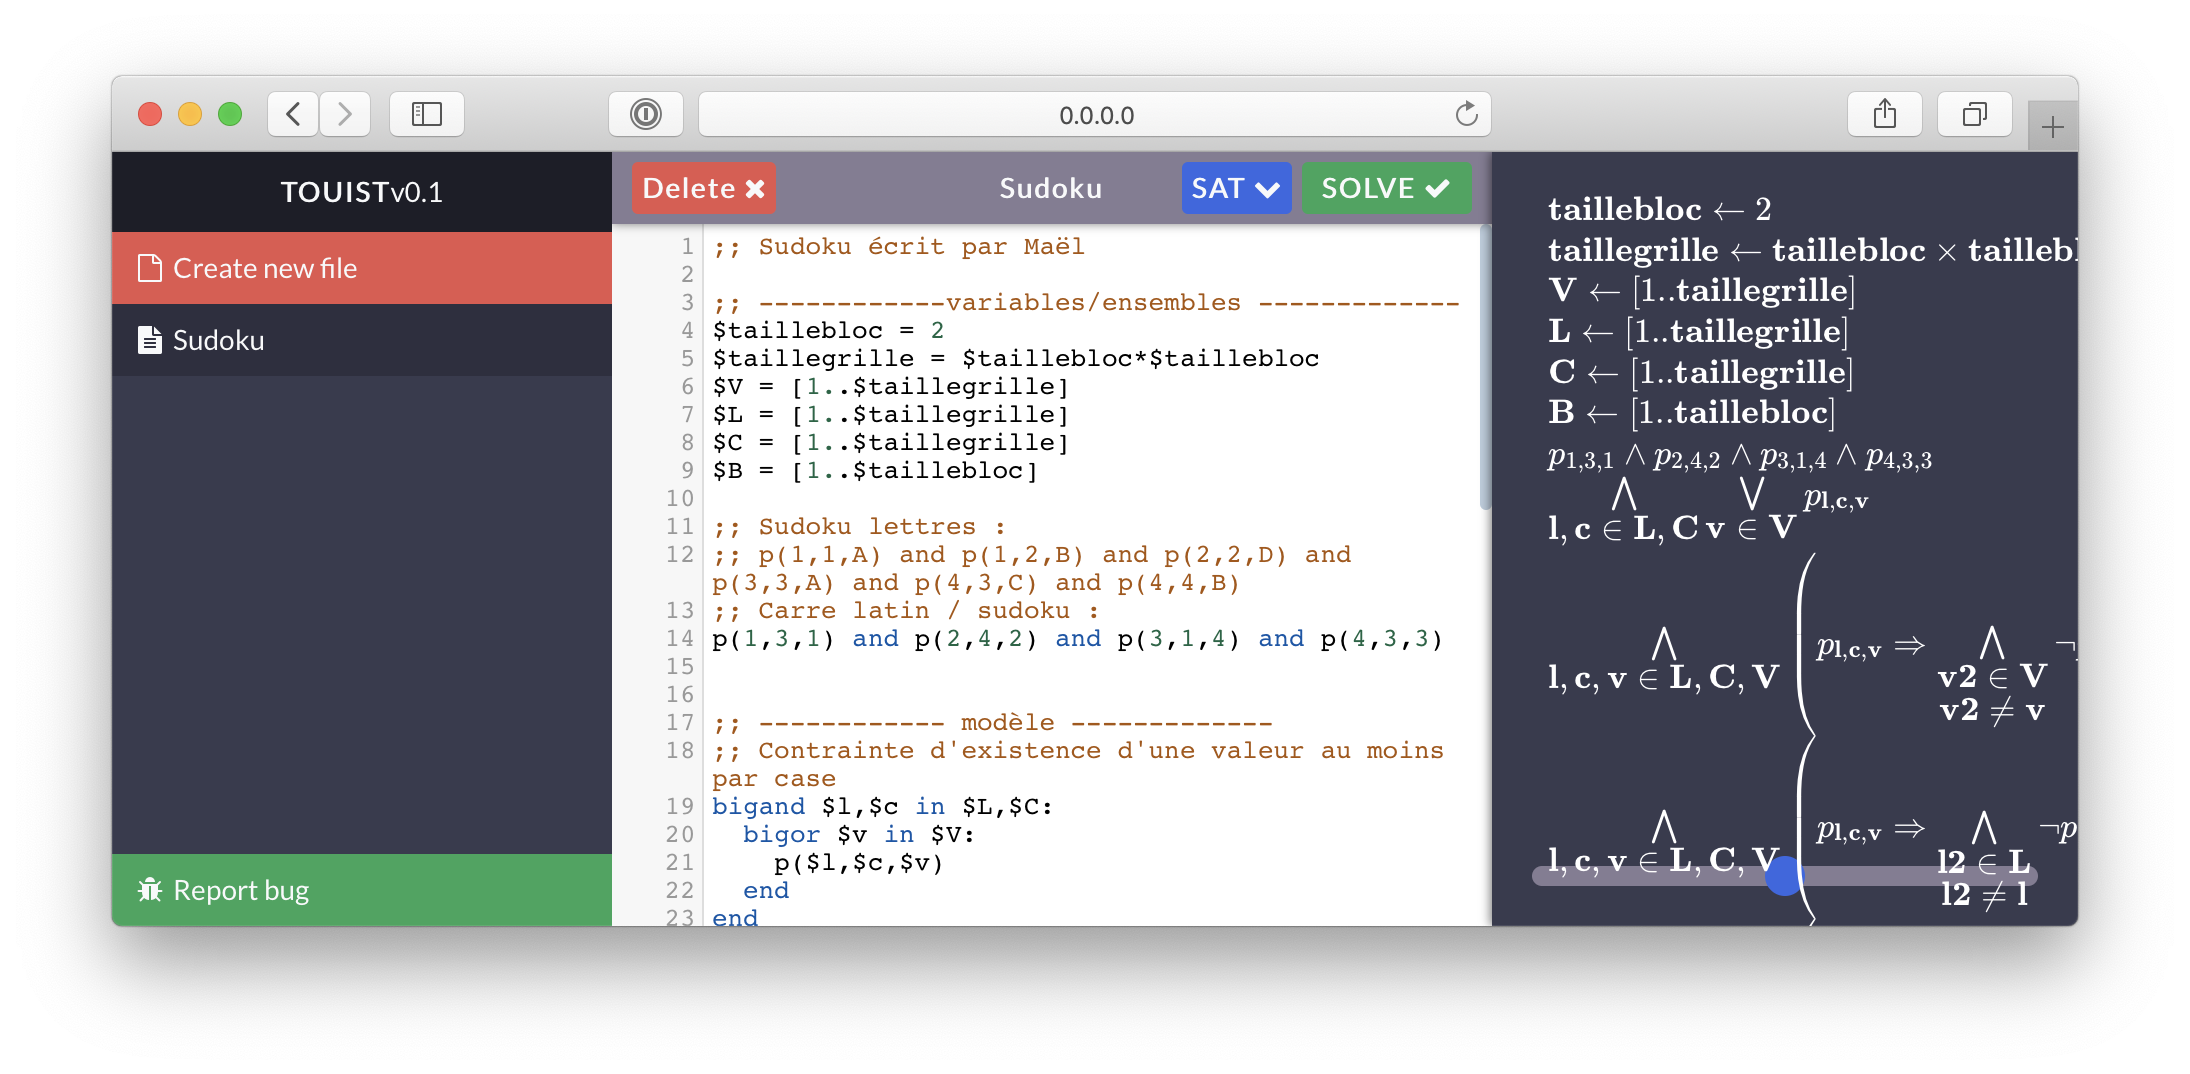
\includegraphics[width=1\textwidth]{figures/touist-web}
  \caption{Application Web pour \touist. Nous projetons de l'utiliser en remplacement de l'application Java.} \label{fig:touist-web}
\end{figure}

\begin{figure}[!ht] \centering
  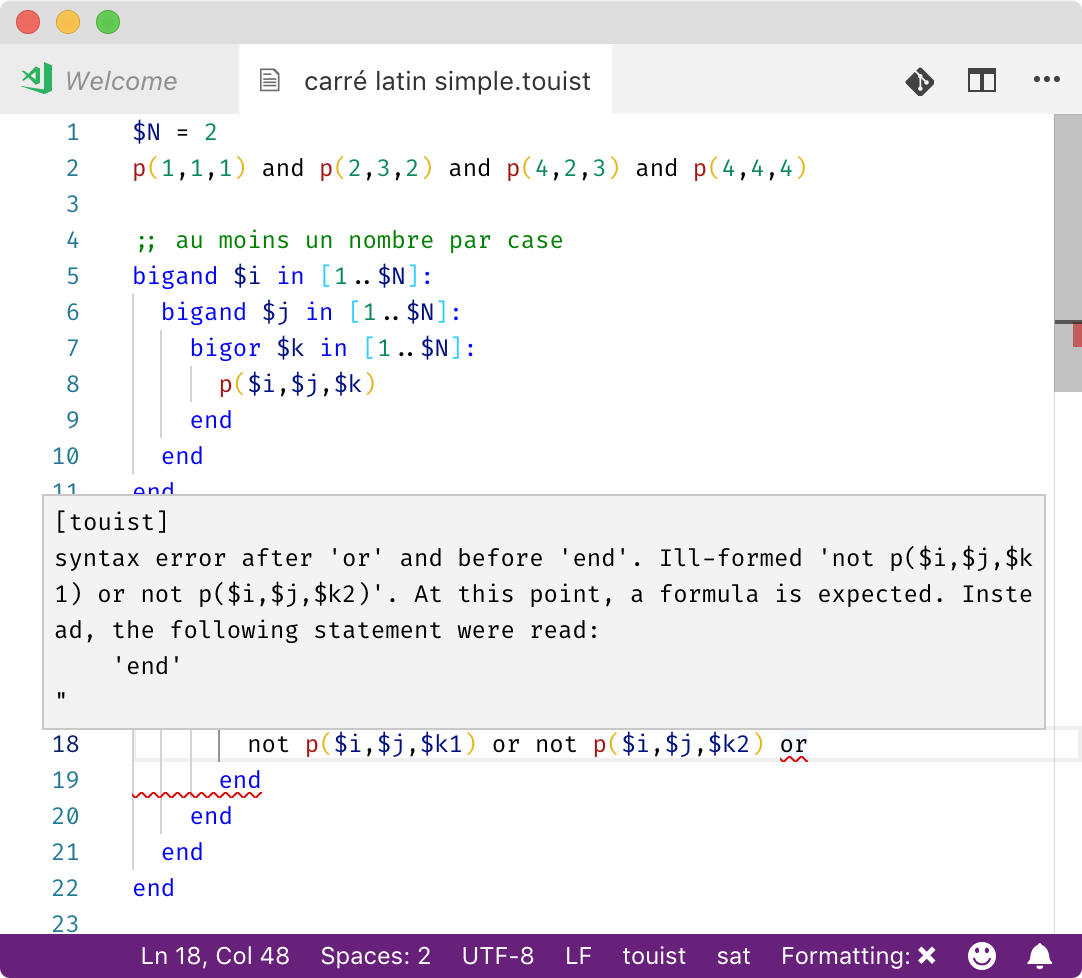
\includegraphics[width=0.7\textwidth]{figures/vscode-touist-white-with-err}
  \caption{\touist peut être utilisé plus confortablement dans un IDE (ici, Visual Studio Code, un éditeur open-source). Une extension permet de voir les erreurs de syntaxe et propose aussi la coloration syntaxique.} \label{fig:touist-vscode}
\end{figure}

\paragraph{Disponibilité des outils}

Le programme \enquote{caché} utilisable en ligne de commande est disponible à la fois sur \href{https://opam.ocaml.org/packages/touist}{OPAM}, le package manager propre à OCaml (similaire à Npm pour Javascript ou Pip pour Python), ainsi que sur \href{https://github.com/touist/homebrew-touist}{Homebrew}, un package manager pour macOS. Ils permettent d'installer l'outil très rapidement et sans connaissances en développement ou compilation :

\begin{verbatim}
    opam install touist
    brew install touist/touist/touist
\end{verbatim}